\begin{figure}[!h]
    \centering
    \minipage{0.5\textwidth}
    \centering
    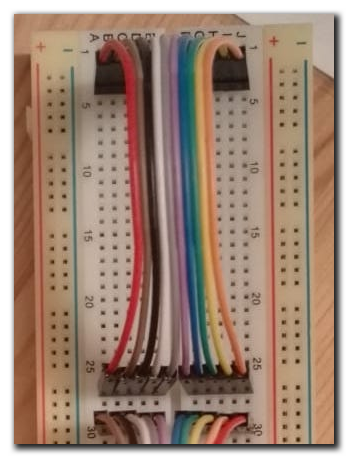
\includegraphics[height=0.67\textwidth]{figures/breadboard}
    \endminipage\hfill
    \minipage{0.5\textwidth}
    \centering
    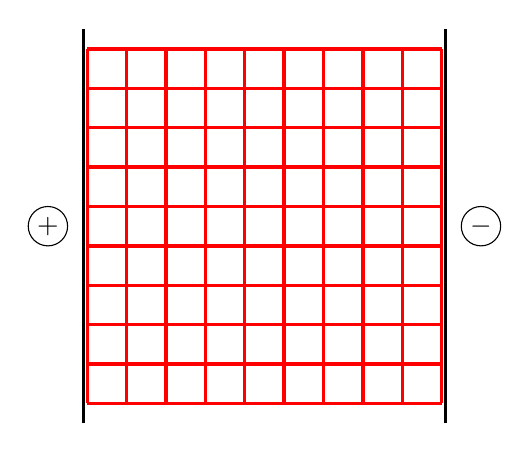
\begin{tikzpicture}
        \foreach \x in {0,0.50,...,4.00} {
            \foreach \y in {0,0.50,...,4.00} {
                \draw[red, very thick] (\x, \y) -- (\x, \y + 0.50);
                \draw[red, very thick] (\x, \y) -- (\x + 0.50, \y);
            }
            \draw[red, very thick] (\x, 4.50) -- (\x + 0.50, 4.50);
            \draw[red, very thick] (4.50, \x) -- (4.50, \x + 0.50);
        }
        \draw (-0.5, 2.25) circle[radius=0.25] node {$+$};
        \draw (5.00, 2.25) circle[radius=0.25] node {$-$};
        \draw[very thick] (-0.05, -0.25) -- (-0.05, 4.75);
        \draw[very thick] (4.55, -0.25) -- (4.55, 4.75);
    \end{tikzpicture}
    \endminipage\hfill
    \caption{The circuit on a breadboard (left) and its schematic diagram (right)}
    \label{fig:breadboard}
\end{figure}

